To improve database performance, we have added indexes \parencite{web:MongoIndexes}. With this, database management system has a faster way to identify location of document in our collection. Listed bellow we can see collections and their indexes.
\begin{center}
\begin{longtable}{ |m{4cm}|m{9cm}| } 
 \hline
 Collections name & Index description \\ 
 \hline
  users &   
  \begin{itemize}
    \item Index type: regular
    \item This collection can benefit on stock index {\_}id. Any other index would not be benefitial at the moment since we are not using this collection a lot. Most of the queries are done by {\_}id.
  \end{itemize} \\
  
  \hline
  iot{\_}customer{\_}devices &  
  \begin{itemize}
    \item Index type: regular
    \item In this collection we have a custom index with the name of UserID. As name suggests, this field has the value from collection users with users ID. Comparison bellow shows that index did not save us much time but on the document examined section, we have navigated straight to our document. If this would be larger database, time would be much bigger concern.
    \item Performance without index
    \begin{itemize}
        \item executionTimeMillis : 2
        \item totalKeysExamined : 0
        \item totalDocsExamined : 1200
    \end{itemize}
    \item Performance with index
    \begin{itemize}
        \item executionTimeMillis : 3
        \item totalKeysExamined : 1
        \item totalDocsExamined : 1
    \end{itemize}
  \end{itemize} \\
  
  \hline
  iot{\_}device{\_}info &  
  \begin{itemize}
    \item Index type: regular
    \item This collection is small (at the moment) and it does not benefit much from indexing. But in case we wanted to index it, we would do it by device type and its manufacturer.
    \item Performance without index
    \begin{itemize}
        \item executionTimeMillis : 0
        \item totalKeysExamined : 0
        \item totalDocsExamined : 1
    \end{itemize}
    \item Performance with index
    \begin{itemize}
        \item executionTimeMillis : 0
        \item totalKeysExamined : 0
        \item totalDocsExamined : 1
    \end{itemize}
  \end{itemize} \\
  
  \hline
 iot{\_}device{\_}history &  
  \begin{itemize}
    \item Index type: regular
    \item History is build as UserID (key): DeviceID (value) and in the DeviceID we have history. The idea was to create a temporary index on UserID. So, when user logs in, index is created in database and when they log out, index is removed. Upon creating index, we have noticed that indexing seems to not be performing as well. In the future, we would break the UserID (key): DeviceID (value) to UserID: value of key and to DeviceID: value of device.
    \item Performance without index
    \begin{itemize}
        \item executionTimeMillis : 37
        \item totalKeysExamined : 0
        \item totalDocsExamined : 53838
    \end{itemize}
    \item Performance with index
    \begin{itemize}
        \item executionTimeMillis : 55
        \item totalKeysExamined : 53838
        \item totalDocsExamined : 53838
    \end{itemize}
  \end{itemize} \\
  \hline
\caption{Indexes on collections}
\end{longtable}
\end{center}

\begin{figure}[H]
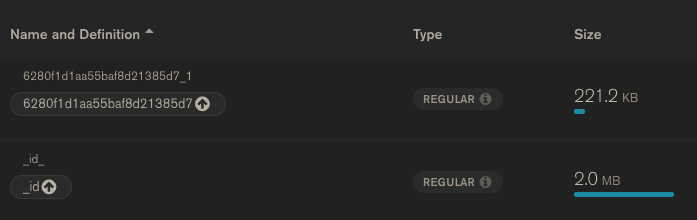
\includegraphics[scale=0.55]{img/iot_device_history-index.jpeg}
\centering
\caption{iot{\_}device{\_}history collection index}
\end{figure}


\begin{figure}[H]
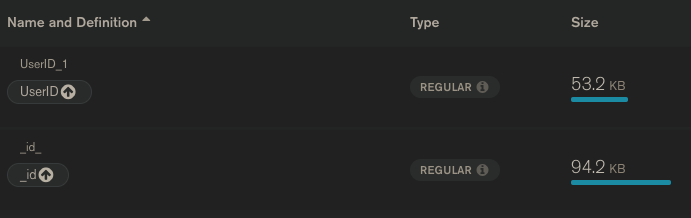
\includegraphics[scale=0.55]{img/iot_customer_devices-index.jpeg}
\centering
\caption{iot{\_}customer{\_}devices collection index}
\end{figure}


\begin{figure}[H]
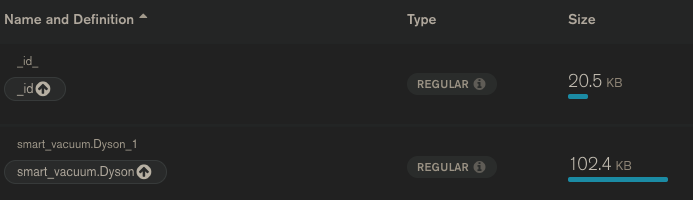
\includegraphics[scale=0.55]{img/iot_device_info-index.jpeg
}
\centering
\caption{iot{\_}device{\_}info collection index}
\end{figure}


\begin{figure}[H]
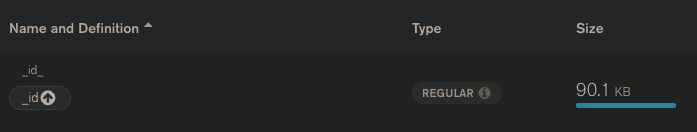
\includegraphics[scale=0.55]{img/users-index.jpeg}
\centering
\caption{users collection index}
\end{figure}
